\section{Bézier curves}\label{sec:bezier-curves}
To achieve a smooth, parametric curve, widely used in computer graphics, animation and font creation, the Bézier curves are used.
They are named after Pierre Etienne Bézier (1910-1999) --- a French engineer and mathematician with merits in the field of mechanical engineering.

The Bézier curves are based on the \textit{Berenstein polynomial basis}, which was "introduced 100 years ago as a means to constructively prove the ability of polynomials to approximate any continuous function, to any desired accuracy, over a prescribed interval"~\cite{farouki2012bernstein}.
In other words, this is the constructive proof of the \textit{Weierstrass theorem} (\textit{approximation theorem}), which "states that the continuous function $f(x)$ on an interval $[a, b]$ and a tolerance $\epsilon > 0$, a polynomial $p_n(x)$ of sufficiently high degree $n$ exists, such that:

\begin{equation}
    \mid f(x) - p_n(x) \mid \leq \epsilon, \quad \forall x \in \left[ a,b \right]\label{eq:weierstrass-error}
\end{equation}

In other words, polynomials can uniformly approximate any function that is merely continuous over a closed interval"~\cite{farouki2012bernstein}.
If so, some of the properties for the Bézier curves are derived immediately, for example, it is known that the basis functions are real, the curve generally follows the shape of the control polygon, the first and last points on the curve are coincident with the first and last points of the control polygon, and so on~\cite{bezier-curves}.

The Bézier curve of $n+1$ control points are defined in~\cite{farouki2012bernstein} as:
\begin{equation}
    r(t) = \sum_{k=0}^n p_k b_k^n(t),  \quad t \in [0,1]\label{eq:bezier-control-points}
\end{equation}

Where the $p_0,\dots,p_n$ are the \textit{control points} and $b_k^n$ is the Berenstein polynomial:
\begin{equation}
    b_k^n(t) = \binom{n}{k} t^k (1-t)^{n-k}, \quad \binom{n}{k} = \frac{n!}{k!(n-k)!}\label{eq:berenstrain-polynomial}
\end{equation}

For example, the two-dimensional Bézier curve is described as a pair of a polynomials:
\begin{equation}
    (x,y) = \left( \sum_{k=0}^n x_{k} b_k^n(t), \sum_{k=0}^n y_{k} b_k^n(t) \right)\label{eq:bezier-point}
\end{equation}

\begin{figure}[h!]
    \centering
    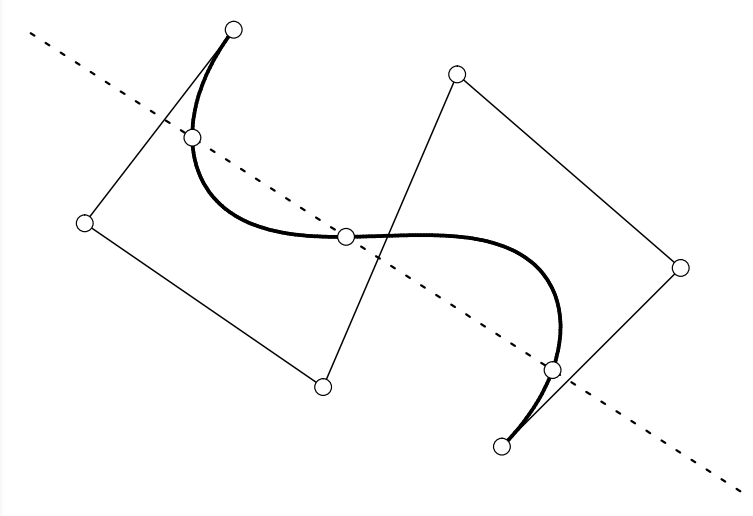
\includegraphics[width=0.4\linewidth,scale=0.4]{resources/bezier-curve-example.png}
    \captionof{figure}{Example of Bézier curve fitting to the control points from~\cite{farouki2012bernstein}}
    \label{fig:bezier-example}
\end{figure}

The control points $p_0,\dots,p_n$ shape the control polygon for the Bézier curve, where the first and the last points on the Bézier curve are coincident with the control polygon (detailed proof and mathematical derivation can be found in~\cite{farouki2012bernstein}).
The properties of the Bézier curve allow for creating the smooth shape, that is going through a set of predefined points and the curve is trying to `follow' the polygon.
This makes this solution convenient from the point of view of this work because the prepared bot is expected to make moves in a human-like manner, so the moves should be smooth and look natural.An example of the control polygon with the Bézier curve shaped by it can be seen in Fig.~\ref{fig:bezier-example} from~\cite{farouki2012bernstein}.
